\documentclass[12pt, twoside]{article}
\usepackage[letterpaper, margin=1in, headsep=0.2in]{geometry}
\setlength{\headheight}{0.6in}
%\usepackage[english]{babel}
\usepackage[utf8]{inputenc}
\usepackage{microtype}
\usepackage{amsmath}
\usepackage{amssymb}
%\usepackage{amsfonts}
\usepackage[nomessages]{fp} %\FPeval{\var-name}{2*sin(pi/6)}
\usepackage{siunitx} %units in math. eg 20\milli\meter
\usepackage{yhmath} % for arcs, overparenth command
\usepackage{tikz} %graphics
\usetikzlibrary{quotes, angles, arrows, arrows.meta}
\usepackage{graphicx} %consider setting \graphicspath{{images/}}
\usepackage{parskip} %no paragraph indent
\usepackage{enumitem}
\usepackage{multicol}
\usepackage{venndiagram}

\usepackage{fancyhdr}
\pagestyle{fancy}
\fancyhf{}
\renewcommand{\headrulewidth}{0pt} % disable the underline of the header
\raggedbottom
\hfuzz=2mm %suppresses overfull box warnings

\usepackage{hyperref}

\fancyhead[LE]{\thepage}
\fancyhead[RO]{\thepage \\ Name: \hspace{4cm} \,\\}
\fancyhead[LO]{BECA / Dr. Huson / Geometry\\*  Unit 9: Dilation and similarity \\* 29 March 2023}

\begin{document}

\subsubsection*{9.8 Classwork: Scaling area and volume \hfill CCSS.HSG.SRT.B.5}
\begin{enumerate}
  \item Dilate rectangle $BECA \rightarrow B'E'C'A'$ by a factor of $k=2$ centered at $(0,0)$.
  \begin{multicols}{2}
    \begin{tikzpicture}[scale=.8]
      \draw [help lines] (-1,-7) grid (7,3);
      \draw [thick, ->] (-1.2,0) -- (7.4,0) node [below right] {$x$};
      \draw [thick, ->] (0,-7.2)--(0,3.4) node [left] {$y$};
      \draw [thick] (2,1)node[above left]{$B$}--
        (3,1)node[above right]{$E$}--
        (3,-3)node[below right]{$C$}--
        (2,-3)node[below left]{$A$}--cycle;
    \end{tikzpicture}

    Find the area of the preimage and image. (show the length times width calculation)\\[5cm]
    By what factor did the area scale?
  \end{multicols}

\item Given $\triangle CAT \sim \triangle NAP$. $CA=14$, $CT=13.3$, $NA=28$, $TP=21$, $m\angle T=80^\circ$, $m\angle NAP = 70^\circ$. Mark the given values on the diagram, find the scale factor, and solve the triangles (all angles and lengths).
  \begin{flushright}
    \begin{tikzpicture}[scale=1.8]
        \draw [thick]
          (-2,0)node[above]{$C$}--
          (0,0)node[above left]{$A$}--
          (4,0)node[below]{$N$}--
          (70:2)node[left]{$P$}--
          (-110:1)node[below right]{$T$}--cycle;
      \end{tikzpicture}
  \end{flushright}

\newpage
\item After a dilation with center $(0,0)$, the image of $\overline{ST}$ is $\overline{S'T'}$. If $ST=8.2$ and $S'T'=28.7$, find the scale factor of this dilation. \vspace{2cm}

\item Regents problem: In triangle $ABC$, points $D$ and $E$ are on sides of $\overline{AB}$ and $\overline{BC}$, respectively, such that $\overline{DE} \parallel \overline{AC}$, and $BD:DA = 3:2$.\\[0.5cm]
If $DB=11.4$ and $DE=12.6$, what is the length of $\overline{AC}$, to the \emph{nearest tenth}?
\begin{flushright}
  \begin{tikzpicture}[scale=0.5, rotate=-11]
    \draw [thick]
    (0,0)node[above]{$B$}--
    (-130:10)node[below]{$A$}--
    (-40:8)node[below]{$C$}--cycle;
    \draw [thick]
    (-130:6)node[above left]{$D$}--
    (-40:4.8)node[right]{$E$};
  \end{tikzpicture}
\end{flushright}


\item In right triangle $ABC$ shown below, point $D$ is on $\overline{AB}$ and point $E$ is on $\overline{BC}$ such that $\overline{AC} \parallel \overline{DE}$. Given $AB=13.2$, $BC=12$, and $EC=7$.
    \begin{enumerate}
      \begin{multicols}{2}
        \item Find the length of $\overline{BE}$. \vspace{1cm}
      \item Find the scale factor, $k$, dilating $\triangle DBE \rightarrow \triangle ABC$, centered at $B$. \vspace{1.5cm}
      \item Find $BD$.
    \begin{center}
      \begin{tikzpicture}[scale=0.55]
        \coordinate [label=above right:$A$](A) at (-12,6);
        \coordinate [label=below left:$B$](B) at (0, 0);
        \coordinate [label=below right:$C$](C) at (-12,0);
        \coordinate [label=above:$D$](D) at (-5, 2.5);
        \coordinate [label=below:$E$](E) at (-5,0);
        \draw [thick] (A)--(B)--(C)--cycle;
        \draw [thick] (A)--(C);
        \draw [thick] (D)--(E);
      \end{tikzpicture}
    \end{center}
  \end{multicols} \vspace{1.5cm}
  \item Find as many other lengths and angle measures as you can.
\end{enumerate}

\end{enumerate}
\end{document}
